% ===== VERSION 2 (2026-09-11): manuscript and supplement titles harmonised (both now "Guidance and surveillance capability for bystander S. aureus tetracycline resistance under doxy-PEP: a three-stream evidence audit"). =====
% JAC Original Article — portable/journal-agnostic LaTeX source.
% TEMPLATE_PENDING: no official JAC/OUP LaTeX class was supplied; migrate this
% source into the official template when obtained. House style verified against
% JAC_IFA.rtf (Instructions to Authors): methicillin (not
% meticillin); MIC in mg/L; sequential superscript references; structured
% NOTE: JAC mandates BRITISH spelling, but the text was converted to US spelling
% at author request; reconcile this before submitting to JAC.
% synopsis (Background optional / Objectives / Methods / Results / Conclusions),
% 250 words; main text (Introduction–Discussion) <= 3500 words; Funding and
% Transparency declarations sections required; figures 88 mm / 180 mm with alt
% text under each legend.
\documentclass[12pt,a4paper]{article}
\usepackage[utf8]{inputenc}
\usepackage[T1]{fontenc}
\usepackage{times}
\usepackage{amsmath,amssymb}
\usepackage{graphicx}
\usepackage{booktabs}
\usepackage{tabularx}
\usepackage[margin=1in]{geometry}
\usepackage{setspace}
\usepackage[right]{lineno}
\usepackage{url}
\usepackage[super,sort&compress,comma]{natbib}
\bibliographystyle{vancouver}
\graphicspath{{figures/}}

\doublespacing
\pagestyle{empty} % JAC: do not insert page numbers
\setlength{\parindent}{0.5cm}

\newcommand{\sa}{\emph{S.~aureus}}
\newcommand{\Sa}{\emph{Staphylococcus aureus}}

\begin{document}

% ---------- TITLE PAGE ----------
\begin{center}
{\Large\bfseries Guidance and surveillance capability for bystander \Sa{}
tetracycline resistance under doxy-PEP: a three-stream evidence audit}\\[1.2em]
\end{center}

\noindent Adrian C. \textsc{Demidont}\textsuperscript{1,2}*\\[0.6em]
\noindent\textsuperscript{1}Nyx Dynamics, LLC, Fairfield, Connecticut, USA\\
\noindent\textsuperscript{2}Nyx Institute for Computational Medicine, Philadelphia, Pennsylvania, USA\\[0.6em]

\noindent\textbf{Running title:} Surveillance and doxy-PEP bystander \sa{} resistance\\[0.6em]

\noindent*Corresponding author. Nyx Dynamics, LLC, Fairfield, Connecticut, USA.
Tel: +1-215-901-2366. E-mail: acdemidont@nyxdynamics.org\\
\noindent ORCID: 0000-0002-9216-8569

\vspace{1.5em}

% ---------- SYNOPSIS ----------
\noindent\textbf{\large Synopsis}

\smallskip
\noindent\textbf{Background.} Doxycycline post-exposure prophylaxis (doxy-PEP)
prevents bacterial sexually transmitted infections and has scaled into guidance
internationally. Doxycycline also selects tetracycline resistance beyond its
target, and \Sa{}---a commensal and pathogen for which doxycycline is one of a
limited number of oral options---is the natural bystander.

\noindent\textbf{Objectives.} To determine whether the guidance and surveillance
deployed around doxy-PEP could follow the bystander-resistance signal the pivotal
trial's final analysis resolved, rather than to estimate a population effect.

\noindent\textbf{Methods.} A reproducible, public-data audit of three evidence
streams---clinical trials, governmental guidance and deployed US
surveillance---each scored against one yardstick: the within-exposed relative
risk it could detect, benchmarked to an empirical colonization estimate.

\noindent\textbf{Results.} The final randomized DoxyPEP analysis reported a
3.89-fold higher hazard of incident doxycycline-resistant \sa{} under doxy-PEP
(95\% CI 1.42--10.68; 68 of 393 versus 5 of 163 incident events), with no effect
on colonization clearance. Yet 0 of 6 outbreak-matched governmental guidelines (0 of 10 coded)
required \sa{} monitoring, and 0 of 12 established US surveillance systems linked
doxy-PEP exposure to an \sa{} tetracycline phenotype at a common population
denominator. Under realistic exposure density and isolate volumes, an ordinary
population system would need an implausible within-exposed effect
(RR~$\approx$~6--28) to move a rate.

\noindent\textbf{Conclusions.} The upstream trial generated information the
downstream architecture is not built to receive. Following the signal requires
sentinel surveillance linking doxy-PEP exposure to the \sa{} tetracycline
phenotype at a common denominator. No population-level causal claim is made.

\vspace{1em}
\linenumbers

% ---------- INTRODUCTION ----------
\section*{Introduction}

Doxycycline post-exposure prophylaxis (doxy-PEP) substantially reduces bacterial
sexually transmitted infections (STIs) and has moved quickly from trial result
into guidance at every level, from the World Health Organization through national
and municipal health departments.\cite{luetkemeyer2023,cdc2024doxypep} Every dose
is selective pressure, and not only on the organisms it targets. \Sa{} is the
consequential bystander: it colonizes the anatomical sites these trials swabbed
and carries mobile tetracycline resistance determinants.\cite{grossman2016} For
two decades, community MRSA in these networks has been documented not as
steady-state carriage but as clustered, outbreak-pattern transmission---the
USA300 lineage moving through sexual networks in San Francisco, Tokyo and
Chicago\cite{diep2008,dejong2025}; the organism colonizing these networks is the
same one carried on skin community-wide, so resistance selected within the
network could, if transmitted, extend beyond it. Tetracycline-resistant USA300
was in fact documented in an MSM-predominant community health population two
decades ago, although by the doxycycline-sparing \emph{tet}(K) mechanism, with
those isolates remaining doxycycline-susceptible.\cite{han2007} Doxycycline is
one of a limited number of oral options for outpatient skin and soft-tissue
infection, a choice often made empirically before any methicillin result
returns,\cite{stevens2014,liu2011} so tetracycline susceptibility can matter
clinically before methicillin status is known.

Clinicians who prescribe doxy-PEP have registered the concern directly: in a
survey of Italian STI-clinic dermatologists, 91.7\% named methicillin-resistant
\sa{} (MRSA) selection as a worry, tied with gonococcal resistance as the
highest-rated,\cite{dona2026} and a systematic review of 1840 healthcare
professionals across four countries likewise placed antimicrobial resistance
among the leading concerns about doxy-PEP.\cite{spence2026} The trial literature has now answered a version of
it. In the final DoxyPEP analysis, among participants free of
doxycycline-resistant \sa{} at baseline, doxy-PEP carried a 3.89-fold higher
hazard of incident doxycycline-resistant \sa{} (95\% CI 1.42--10.68; 68/393
versus 5/163; $P=0.0044$), while the hazard of clearing colonization did not
differ between arms (HR 1.01, 0.69--1.46).\cite{luetkemeyer2025} The trial's
authors called for public-health surveillance of antimicrobial resistance (AMR)
in \sa{} and other commensals.

That call defines the present question. We ask not whether doxy-PEP drives
population-level resistance---a claim we do not make---but whether the guidance
and surveillance deployed around doxy-PEP could follow the signal the trial
resolved, at the population level where the clinical stake lies. The clinically
decisive axis is tetracycline (doxycycline) susceptibility used in empirical oral
therapy, not the methicillin axis around which staphylococcal surveillance is
organized. We audit the three places an answer would have to come from---the
trials, the guidance and the deployed surveillance---each against a single
detectability yardstick.

% ---------- MATERIALS AND METHODS ----------
\section*{Materials and methods}

\subsection*{Design}
The study is a documentary and quasi-computational audit assembled in three
streams, collected and analyzed in sequence: clinical trials (Stream A), the
governmental guidance built on them (Stream B) and the population surveillance
meant to monitor them (Stream C). No individual-level or restricted data were
used; every input is public, so no ethical approval was required. Sources were
located, read, coded with page/section/table locators and SHA-256-pinned before
analysis; analysis decisions that could go either way were date-logged before
results were known; and every figure and table regenerates from a single command
over a test-gated pipeline archived with a citable
DOI.\cite{armond2024integrity} A large language model assisted with writing and
analysis engineering; the author verified every numerical value and quotation
against primary sources and takes full responsibility (see Acknowledgements).

\subsection*{Detectability yardstick}
Each stream is scored on one commensurable quantity: the within-exposed relative
risk (RR) it could detect. The empirical benchmark is Soge \textit{et
al.}\cite{soge2025} (tetracycline-resistant \sa{} colonization, 18\% versus 8\%
in doxy-PEP users with $>$3 doses/month versus non-users; RR~$\approx$~2.25); a
cross-organism gonococcal RR~$\approx$~1.42 is carried as a flagged, more
conservative secondary. Because the randomized trial reports a within-exposed
hazard ratio of 3.89, well above this band, the detectability verdict below is
invariant to which anchor is used: the relative risk a population system would
need to see (RR~6--28, Results) exceeds both the cross-sectional benchmark and
the trial's own hazard ratio.

\subsection*{Sources and coding}
The author identified, retrieved and screened all source documents for
eligibility; each eligible document was then coded from full text against a
prespecified schema, every value carrying a page, section or table locator. For
the guidance corpus (Stream B), two independent machine (large language model)
passes coded each document under separate blinded prompts, and disagreements were
resolved by the author against the source. Per-field agreement is reported as raw
concordance, which measures the reproducibility of the coding protocol rather
than independent human adjudication; a Cohen's $\kappa$ is given for context only,
with the caveat that the two passes share a model lineage and are therefore not
fully independent (Limitations). The surveillance enumeration (Stream C) was
coded by a single pass; its inclusion and exclusion list, with a stated reason
per system, is given in the Supplementary data and reflects systems as deployed
as of August 2026. All coding prompts and outputs are in the public repository.

\subsection*{Stream A---trials}
For each primary-trial \sa{} arm comparison (first-party published data only), we
computed, from arm sizes and observed control rate, the exact (Fisher) power to
detect the externally fixed benchmark effect and the minimum detectable RR at
80\% power; fixing the effect externally makes this a design-based sensitivity
analysis rather than observed power. The \sa{} assay is doxycycline throughout
(E-test, MIC~$\geq$~16~mg/L). We tabulated how the resistance result was reported
across trial venues and secondary syntheses (numerator, denominator basis,
conditioning set and terminology). The final trial performed the appropriate
participant-level time-to-event test itself; we cite that randomized result
directly and did not re-estimate it. Cross-sectional carriage cannot resolve the
clustered transmission structure of \sa{} in these networks; the supporting
dispersion, trend-test degradation and outbreak-shape analyses are MRSA-scoped
(MRSA being a subset, not the analytic unit) and are reported in the
Supplementary data (available as Supplementary data at \textit{JAC} Online).

\subsection*{Stream B---guidance}
To make the denominator principled, we anchored it to the same clustering
evidence used in Stream A: US jurisdictions with documented community-associated
MRSA/USA300 transmission in men who have sex with men.\cite{dejong2025,diep2008}
We took governmental public-health guidance only (clinic and
provider-organization documents excluded, with reasons). Each document was coded
from full text, one record per document, every finding carrying a locator, for
whether it requires, suggests or omits \sa{} monitoring and whether it names,
counsels on or measures the organism (coding provenance above). An independence
check separated genuinely independent declines from documents that defer to, or
are adapted from, one another.

\subsection*{Stream C---surveillance}
We enumerated a closed universe of established US governmental surveillance
systems (federal, state or metropolitan) that could plausibly capture, at a
population denominator, either doxy-PEP/doxycycline exposure or \sa{} AMR
phenotype, and coded each on three capabilities: exposure-side capture,
phenotype-side capture (of the \sa{} tetracycline unit, not the MRSA subset) and
the join, recording the geographic resolution of each side. A supporting analysis
asked whether, even at a common denominator, the exposed subgroup is dense enough
to move a population rate. The exposed population is indexed on the combined PrEP
and people-living-with-HIV male count (primary specification; the trial enrolled
both, AIDSVu 2024 state PrEP and prevalence), so the dilution fraction is
$f=\phi\,((\text{male-PrEP}+\text{male-PLWH})\ \text{density}/10^{5})\,\text{uptake}\,d\,\kappa$,
where $d$ is the share of users taking $>$3 doses/month (the subgroup carrying the
benchmark effect) and $\kappa$ the isolate-enrichment factor; $f$ is
population-independent
because it tracks exposure density, not headcount, and the minimum detectable
change in a proportion near baseline $R_0$ inverts to
$\mathrm{RR_{needed}}=1+\mathrm{MDE}/(f R_0)$. Parameters were not uniformly
generous: isolate volume was set generously high (favoring detection), while the
realistic under-sampling ($\kappa=0.5$) and dose-threshold ($d=0.5$) factors bound
against it. Both ranges and the resulting $\mathrm{RR_{needed}}$ are reported;
full grids and the metropolitan break-even are in the Supplementary data.

% ---------- RESULTS ----------
\section*{Results}

\subsection*{Stream A: trial measurement and reporting of the \sa{} endpoint}
When the analysis matched the question, the signal appeared. The final DoxyPEP
analysis ran the participant-level test the interim had not---time to first
detection of doxycycline-resistant \sa{} by arm, standard-of-care censored at
crossover, by Cox proportional hazards---and returned HR 3.89 (95\% CI
1.42--10.68; $P=0.0044$), with colonization clearance unchanged (HR
1.01).\cite{luetkemeyer2025} The 2023 interim, by contrast, was presented as reassuring
on a cross-sectional resistance fraction and was underpowered for any externally
specified effect (0 of 4 comparisons powered; minimum detectable RR 3.8--5.1
against the benchmark 1.42--2.25). The hazard ratio is not comparable to that
cross-sectional minimum: the estimand, not the sample size alone, became adequate
to the question.

Two measurement features of the interim record persist and matter downstream.
First, a unit mismatch: the trial's data table is headed ``phenotypic resistance
to the tetracycline antibiotic class'' while its methods define the \sa{} assay
as doxycycline, and the federal guideline then describes the doxycycline result
as ``tetracycline resistance in \sa{}''.\cite{cdc2024doxypep} Because efflux and
ribosomal-protection mechanisms differ in whether doxycycline still works
(below), an endpoint scored as ``the tetracycline class'' does not answer the
treatment-relevant question. Second, the signal was reported over differing,
incompletely documented denominators and then propagated into secondary reporting
under further contrasts (Table~\ref{tab:propagation}): the resistant numerator
changes from 5 to 16 to 28 and the denominator basis shifts from colonized
carriers to all-swabbed, while the percentage travels more reliably than the
denominator, contrast and terminology needed to interpret it. The individual-level
data that could reconcile these first-party reports are not publicly
available.\cite{luetkemeyer2023} Even the intensively surveilled gonococcus was
phenotyped in fewer than one diagnosis in five (resistance testing unavailable for
83\%, 212/256).\cite{luetkemeyer2023croi}

Across trials the phenotype was measured on incompatible terms: DoxyPEP measured
doxycycline resistance by E-test over two denominators; DuDHS measured it by disc
diffusion in single-digit carriers; DOXYVAC measured only MRSA carriage---a
methicillin, not a tetracycline, quantity, and one that itself rose within the
doxy-PEP arm (1.8\% to 9.9\%) while being reported as a between-arms
null.\cite{vanbaelen2024c} A pooled estimate is not defensible, and the
heterogeneity is itself a finding. The trial resolved the doxycycline phenotype
but not its molecular basis---efflux (\emph{tet}(K)) versus ribosomal protection
(\emph{tet}(M))---which a single breakpoint cannot separate.\cite{liu2011,grossman2016}

\begin{table}[t]
\centering
\caption{Propagation of the DoxyPEP \sa{} resistance signal across reporting
venues. Rows are not assumed to be identical estimands; differences in contrast,
conditioning set, denominator and terminology are the object of comparison.}
\label{tab:propagation}
\small
\begin{tabularx}{\textwidth}{@{}lllX@{}}
\toprule
Venue & Reported result & Frame / conditioning set & What travels downstream\\
\midrule
NEJM appendix\cite{luetkemeyer2023} & 5/31 = 16\% & Month-12 doxy-PEP arm; resistant among carriers & Numerator and carrier denominator explicit\\
CROI abstract\cite{luetkemeyer2023croi} & 16/137 = 12\% & Doxy-PEP arm; all-swabbed denominator & Different numerator/denominator basis\\
CDC guideline\cite{cdc2024doxypep} & 28/222 = 13\%; summarized 5\%$\rightarrow$13\% & Doxy-PEP arm; guideline frame & Percentage retained, provenance less transparent\\
JAMA Insights\cite{mayer2023} & 5\% versus 4\% & Doxy-PEP versus control; ``infected with'' & Between-arm percentage only; counts/timepoint dropped\\
JAMA Synopsis\cite{flores2025} & 5\%$\rightarrow$16\% & Within arm, among \sa{}-isolated & Carrier-conditioned within-arm percentage (baseline to month 12)\\
Lancet ID final\cite{luetkemeyer2025} & HR 3.89 (1.42--10.68); 68 of 393 vs 5 of 163 & Participant-level time-to-event; baseline-negative, as-randomised & Not cited by any coded guidance, including two revised after its March 2025 online publication\\
\bottomrule
\end{tabularx}
\end{table}

The estimand shift did not propagate downstream: no guidance document in the
corpus cites the final time-to-event analysis or any hazard ratio, and the two
documents revised after its online publication in March 2025---WHO (2026) and San
Francisco (May 2026)---retained a cross-sectional or generic frame. Non-citation
is telling here because this corpus demonstrably transmits numbers when it has
them: CDC carried the cross-sectional 5\%$\rightarrow$13\% figures and WHO cites
Soge's colonization estimate.\cite{soge2025}

\subsection*{Stream B: \sa{} monitoring requirements in governmental guidance}
The governmental guidance shows a consistent within-document asymmetry: the
efficacy question received a graded, systematic evidence review, while the
AMR-harm question---explicitly including resistant-pathogen development---received
an ungraded review in the same document. Of the six documented-outbreak
jurisdictions with governmental doxy-PEP guidance (San Francisco, Chicago, New
York City, Boston/Massachusetts, Los Angeles County and San Diego), 0 require or
suggest \sa{} monitoring. The decline is not an artifact of copying: four
jurisdictions are independently authored, one (Los Angeles County) is adapted
from San Francisco and one (Massachusetts) from an external template. Nor is it
for want of naming the organism---three of the six name \sa{} specifically, two
invoke only a generic ``microbiome'' risk and one is silent; even where named,
none measure it. Across the full coded corpus (10 documents: CDC, WHO and eight
US jurisdictions) the result is identical: 0 instrument the bystander. Raw
agreement between the two coding passes was 92\%; the single field with meaningful
disagreement ($\kappa=0.58$, context only) is reported unrounded. Providers are nonetheless required to counsel patients about
resistance in commensal organisms---a harm no system measures.

\subsection*{Stream C: surveillance capability and exposure--phenotype linkage}
Following the signal requires one system to carry, at a common population
denominator, both who is exposed to doxy-PEP and what tetracycline phenotype \sa{}
carries. Across the closed universe of twelve established US systems, none does
(Figure~\ref{fig:linkage}). Two systems capture exposure at a population
denominator (AIDSVu and CDC AtlasPlus, as a pre-exposure prophylaxis proxy, not
doxy-PEP itself),\cite{aidsvu} and zero capture \sa{} tetracycline resistance at a
population denominator: the join is vacuous because one half does not exist.

The absence is a codified seam. Wherever \sa{} is surveilled at a population
denominator the reported axis is methicillin: the one population-based platform,
Active Bacterial Core surveillance/Emerging Infections Program (ABCs/EIP),
reports invasive MRSA; the National Healthcare Safety Network reports MRSA events;
and the only routine source of \sa{} tetracycline susceptibility, the facility
cumulative antibiogram, is non-standardized and carries no population
denominator, because CLSI M39 mandates the MRSA/MSSA split and makes tetracycline
a selectively suppressible supplemental agent. The National Antimicrobial
Resistance Monitoring System excludes \sa{} altogether; tetracycline-resistant
\sa{} is nationally notifiable nowhere. Exposure exists at county/metro
resolution and phenotype only at denominator-free facility level, so no geography
carries both. A system could be built---most directly by adding \sa{} tetracycline
susceptibility to ABCs/EIP, which already holds the denominator---but none is
deployed.

Nor could an ordinary population system recover the missing side by collecting
more isolates. Indexing the exposed population on the combined PrEP and
people-living-with-HIV male count---the primary specification, because the trial
enrolled both (Materials and methods)---the realistic-cell within-exposed effect
required to move a population rate runs to RR~$\approx$~6--28 across the
design-effect range (Figure~\ref{fig:detect}); the more restrictive PrEP-only
indexing gives RR~$\approx$~14--64, which overstates infeasibility. Either way it
is far above any plausible effect. Detection appears in a single
cell of the entire grid, where every generous assumption is maxed at once (55\%
uptake, $5\times$ enrichment, 13\% baseline, $100\,000$ isolates/geography-year
and optimistic panel independence): there $\mathrm{RR_{needed}}$ falls to 1.03,
and under single-comparison inference even the most favourable cell stays above
the yardstick (1.79). The verdict thus turns on parameters no deployed system
reports---exposure density, isolate enrichment and dosing frequency---which is the
measurement gap in miniature: the metropolitan best cell needs $1.8\times$ the
combined male exposure density of the densest US geography, and realistic cells
hundreds of times it. The only configuration that restores sensitivity is to
sample \sa{} directly from doxy-PEP-exposed persons, which converts surveillance
into a sentinel cohort.

\begin{figure}[t]
\centering
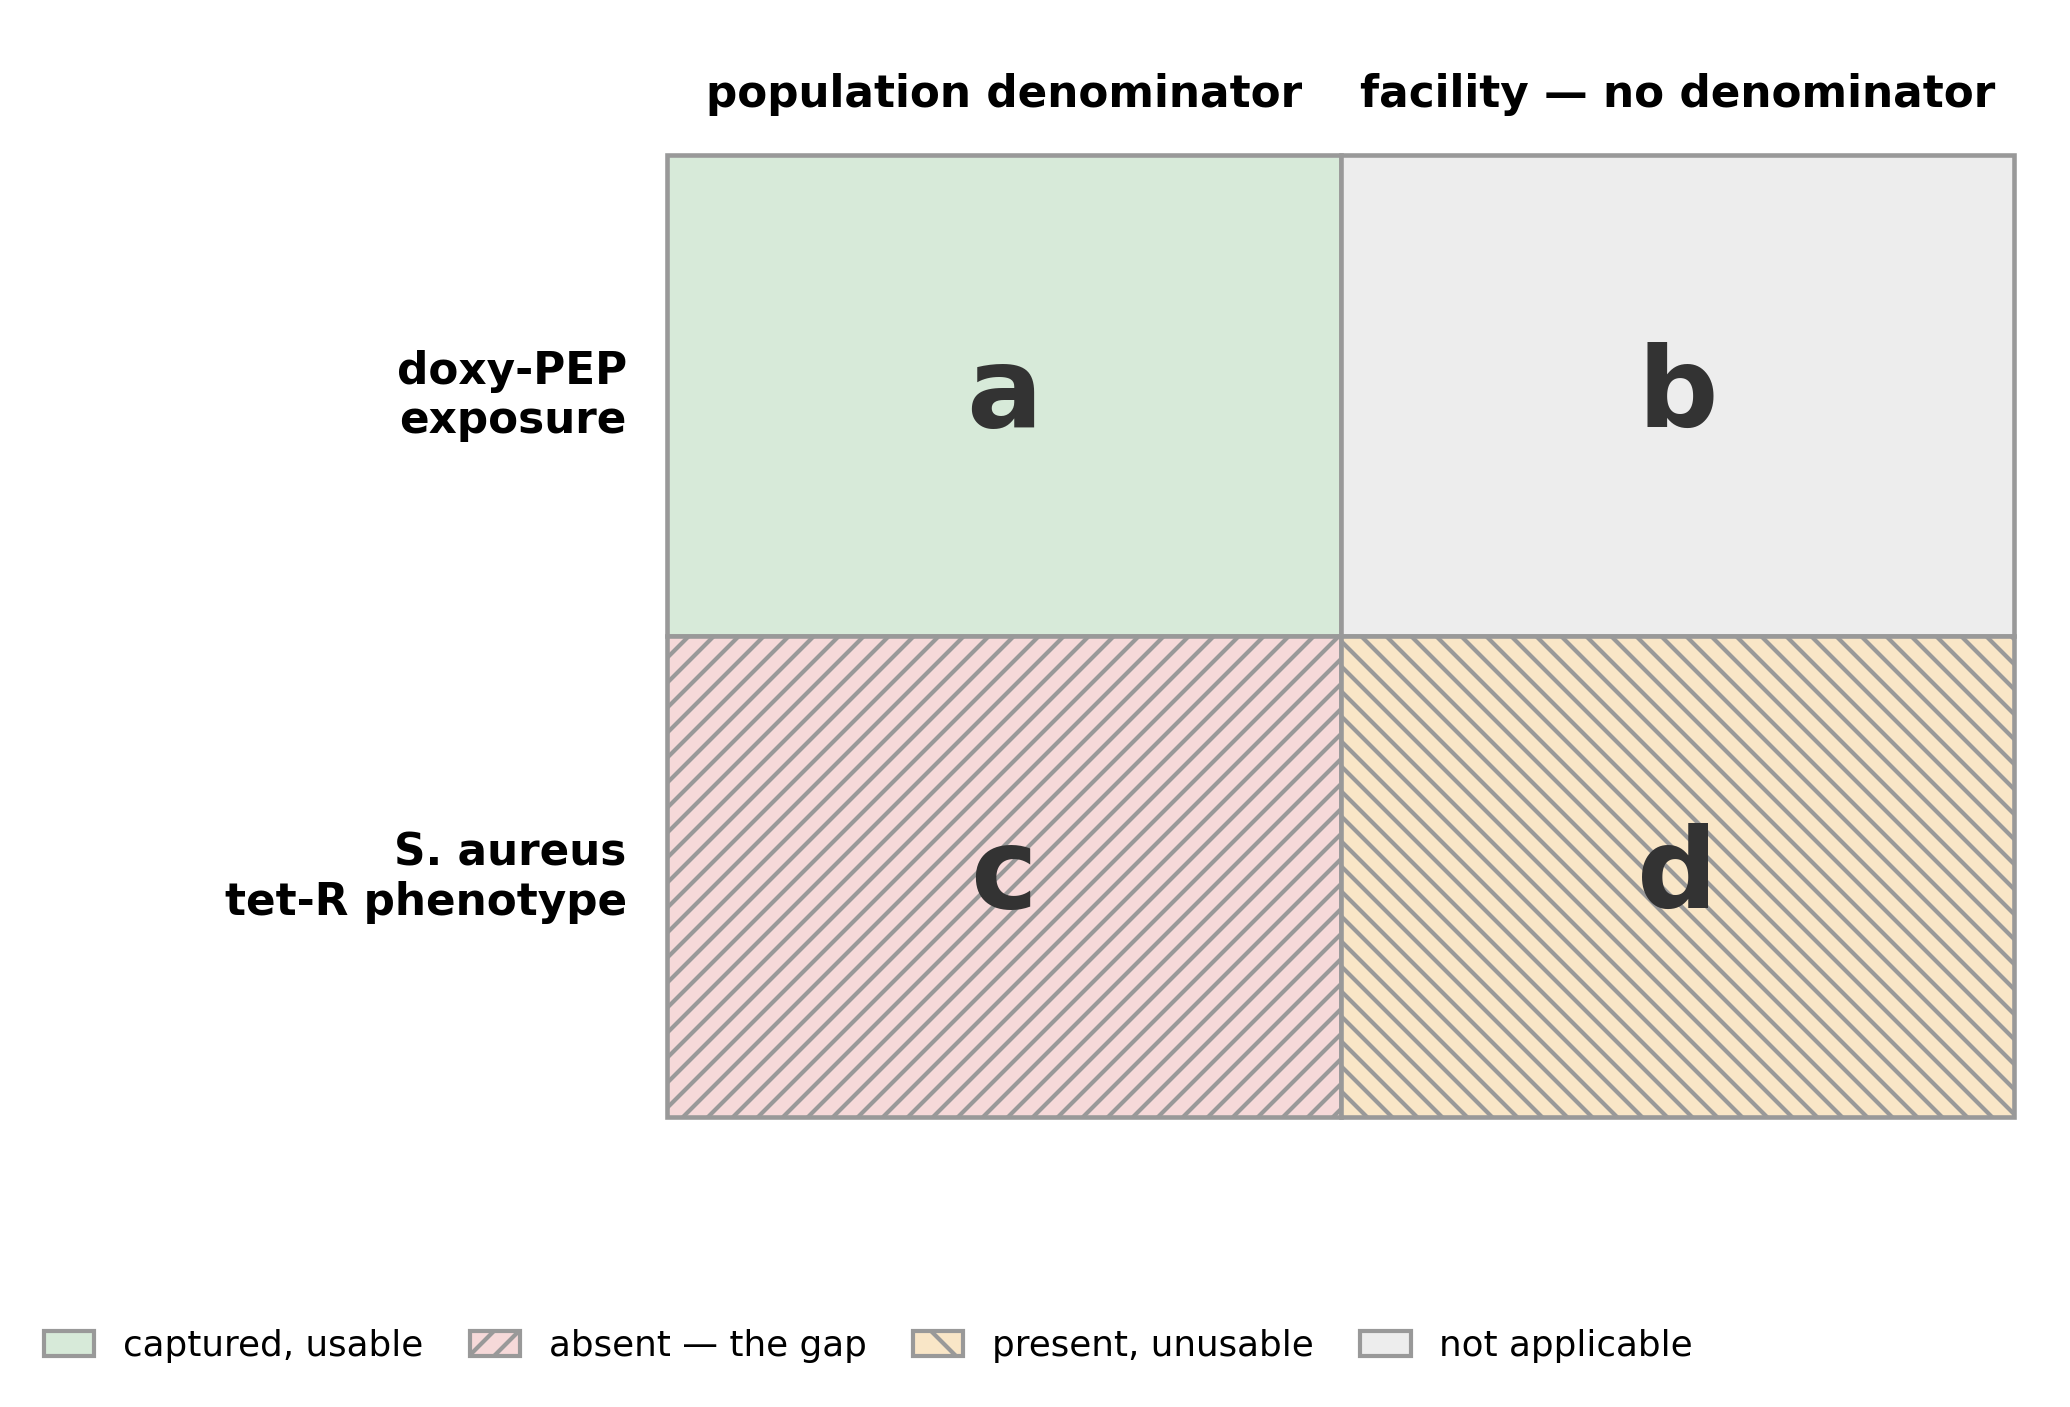
\includegraphics[width=0.9\textwidth]{streamc_linkage.png}
\caption{No deployed US system links doxy-PEP exposure to \sa{} tetracycline
resistance at a common population denominator. Linking the two requires one
column usable in both the exposure and phenotype rows; none is. Exposure is
captured only as a PrEP proxy (AIDSVu, CDC AtlasPlus); the \sa{} tetracycline
phenotype is captured at a population denominator nowhere, because the one
population-based platform reports the methicillin (MRSA) subset. Of 12 systems, 0
join the two.}
\label{fig:linkage}
\end{figure}
\noindent Alt text: A matrix of twelve US surveillance systems against exposure
and phenotype capability; shading shows that exposure is captured only as a PrEP
proxy and the \sa{} tetracycline phenotype is captured at a population
denominator nowhere, so no column links both rows.

\begin{figure}[t]
\centering

\includegraphics[width=0.9\textwidth]{three_streams.png}
\caption{One axis---within-exposed relative risk (log scale)---carries all three
streams against the plausible benchmark band (RR 1.42--2.25). The trial's
resolved effect (HR 3.89) clears the band; guidance requires no \sa{} measurement
so no detection threshold exists; and deployed surveillance would need
RR~$\approx$~6--28 to move a population rate (combined PrEP+PLWH exposed
denominator; the more restrictive PrEP-only indexing gives 14--64). The signal is
above the line while the systems built to follow it are not.}
\label{fig:detect}
\end{figure}
\noindent Alt text: A logarithmic relative-risk axis with a shaded benchmark band
at 1.42 to 2.25; the trial hazard ratio 3.89 sits above the band, surveillance
detectability thresholds of about 14 to 64 sit far to the right, and guidance has
no threshold.

\subsection*{Literature coverage of the bystander organism}
A defined PubMed search (2015--2026) identified 361 doxy-PEP papers, of which 13
(3.6\%) mention a bystander staphylococcal organism and only 2 measure
tetracycline-resistant \sa{} against a doxy-PEP exposure contrast. The bystander
is rarely mentioned and, when mentioned, rarely measured against exposure---the
research attention concentrated where the existing instruments already point.
Table~\ref{tab:audit} summarizes the three streams against the yardstick.

\begin{table}[t]
\centering
\caption{Headline audit of the doxy-PEP evidence base against one detectability
yardstick. Each cell is licensed by the Results above; no composite score is
implied.}
\label{tab:audit}
\small
\begin{tabularx}{\textwidth}{@{}lXl@{}}
\toprule
Stream & Question & Result\\
\midrule
A. Trials & Was the bystander signal resolved? & Yes---HR 3.89 (1.42--10.68), incident doxy-R \sa{}\\
B. Guidance & Is \sa{} monitoring required? & No---0/6 outbreak-matched; 0/10 coded\\
C. Surveillance & Is exposure linked to phenotype? & No---0/12 systems; RR$_{\text{needed}}\approx$6--28 to detect\\
\bottomrule
\end{tabularx}
\end{table}

% ---------- DISCUSSION ----------
\section*{Discussion}

The pivotal trial has now resolved the bystander question it was long thought
unable to reach: a significant increase in incident doxycycline-resistant \sa{}
under randomized exposure, with no matching effect on carriage, and a call from
its authors for surveillance of exactly this.\cite{luetkemeyer2025} The upstream
instrument generated the information. Across the two systems that would have to
receive it---guidance and deployed surveillance---the answer is that they cannot:
guidance instruments nothing (0/6; 0/10) and no deployed system joins exposure to
the \sa{} tetracycline phenotype at a common denominator (0/12).

The sharper reading is that the trial's own measurement system evolved to meet
its internal question while the implementation system did not. The 2023 interim
was presented as reassuring; the 2024 guideline appended a call
for monitoring; the 2025 final analysis asked the estimand the others had not and
returned HR 3.89. Three years, one underlying phenotype, an evolving
estimand\cite{montoya2025estimand}---and, at the end, a demonstrated signal handed
to systems built to measure something else.

\subsection*{Tetracycline resistance mechanisms and the phenotype unit}
Staphylococcal surveillance is standardized around methicillin at every tier,
yet the treatment-relevant axis here is tetracycline susceptibility, used
empirically before methicillin status is known. The two are not
interchangeable, and neither is the molecular basis of tetracycline resistance:
\emph{tet}(K) efflux leaves doxycycline largely usable, whereas \emph{tet}(M)
ribosomal protection can compromise it, and the trial resolved incident
doxycycline resistance without resolving which.\cite{liu2011,grossman2016} The
distinction is not academic. In a national surveillance population of 823 invasive
USA300 isolates, 72 (9\%) were tetracycline-resistant, yet 69 were
doxycycline-susceptible and carried \emph{tet}(K) while only 3 were
doxycycline-resistant and carried \emph{tet}(M)\cite{mcdougal2010}: a single
tetracycline breakpoint reports one number for two clinically opposite
situations. The mechanisms also differ in mobility---\emph{tet}(M) is
characteristically carried on Tn916-like conjugative transposons whose host range
includes \emph{S. aureus} and which transfer across strain boundaries by
cell-to-cell contact,\cite{roberts2011} while the \emph{tet}(K) efflux determinant
is typically plasmid-borne\cite{han2007,mcdougal2010}---so a clonally indexed
system can track a lineage faithfully and still miss a determinant moving between
lineages. An exposure cohort shows the same blindness directly: among 168
military personnel, doxycycline antimalarial prophylaxis was not associated with
overall tetracycline-class resistance in \emph{S. aureus}, yet \emph{tet}(M) genes
were significantly more common in the exposed (p=0.031)\cite{mende2016}---the
aggregate phenotype null while the determinant distribution moved under exposure
(a military, antimalarial-dosed cohort, not doxy-PEP). A surveillance variable can
remain valid for the question it was designed to answer while being insufficient
for the one now imposed on it. We do not forecast which
mechanism is spreading; the point is that the inherited variable cannot say.

\subsection*{Instrument requirements for population monitoring}
Following the signal to the population requires an instrument the deployed
architecture does not provide: sentinel sampling of \sa{} from doxy-PEP-exposed
individuals, which raises the exposed fraction by construction and fixes the
denominator; sampling that includes the oropharyngeal and peri-anal sites, since
nares-only screening under-detects colonization by about 20\% in this
population\cite{kyaw2012}; resistance reported per carrier and by mechanism
(\emph{tet}(M) versus \emph{tet}(K)) rather than as a pooled tetracycline-class
rate; dosing frequency rather than prescription status; a feed carrying \sa{} tetracycline
susceptibility at a population denominator, most directly by adding it to the
platform that already tracks invasive MRSA and joining it to exposure on
geography; and access to individual-level trial data. None is exotic; none
is in place at scale.

These failures share a structure. A guideline or a surveillance system carries in
its sampling frame, cadence, coding, denominator and unit the organism and
question it was built for. The doxy-PEP apparatus was built to measure gonococcal
efficacy; applied to a bystander commensal it inherits a denominator the
intervention itself moves, a phenotype label spanning two mechanisms, and a
surveillance architecture standardized around methicillin while the tetracycline
unit falls orthogonally through it. We call this \emph{measurement inheritance}: a
downstream system retains the dimensions---estimand, denominator, unit, cadence,
linkage, measurement responsibility---appropriate to the upstream question but not
those the downstream question requires, so the question becomes unanswerable not
for want of data but for want of an inherited dimension. It is built from
familiar parts---construct validity, estimand mismatch, ascertainment and
surveillance bias,\cite{tancredi2024surveillance} metric substitution of the
Goodhart type\cite{treem2023visibility}---but concerns how such mismatches couple
\emph{across} stages of an evidence chain. The downstream gap is therefore not
closable by a better analysis of the trial's data---that analysis has been done,
and it is significant---but is a property of the guidance and surveillance
instruments.

Doxy-PEP's benefit accrues to the recipient; the tetracycline selection cost
falls on people outside the prescribing decision---the outpatient with a skin
infection and, at the sharp end, dialysis, surgical and oncology patients for whom
an oral anti-staphylococcal agent is no convenience. A negative externality that
no deployed instrument can price is not thereby small; it is unweighable. The
wider distributive argument---that the two sides are observed on unequal terms, a
property we term \emph{distributive observability}---is developed in the
Supplementary data (S6).\cite{montoya2025affected}

\subsection*{Limitations}
We make no population-level causal claim and no transmission claim: whether the
individual-level signal propagates into a population externality is precisely what
no deployed system can determine. The trial's own randomized result is
significant and we accept rather than dispute it; our earlier aggregate
reconstruction of the interim is retired in its favor. Colonization is not
infection, and the colonization--infection link is itself unmeasured here. Much of
the evidence for how \sa{} clusters and moves through these networks exists only
for its MRSA subset, so where our clustering analysis relies on MRSA we mark it as
such---an instance of the inherited limitation, not an exception to it. Finally,
the trial reaches only a roughly twelve-month horizon; persistence, dose--response
and mechanism remain open. Our coding carries two acknowledged asymmetries: the
guidance corpus was double-coded by two machine passes that share a model lineage
(reported as raw concordance, not independent human adjudication), while the
surveillance enumeration was coded by a single pass. Consistent with a
falsification standard set in advance, the inheritance claim fails if a doxy-PEP
guideline comes to require
\sa{} monitoring, or if a deployed system links doxy-PEP exposure to an \sa{}
tetracycline phenotype at a common population denominator.

\subsection*{Conclusions}
The randomized instrument generated a bystander-resistance signal that the
guidance and surveillance built around doxy-PEP are not instrumented to follow.
The gap is one of measurement architecture, not of missing data, and it is
closable---by sentinel surveillance that links doxy-PEP exposure to the \sa{}
tetracycline phenotype at a common denominator. Until it is built, the population
question the trial's authors posed cannot be run.

% ---------- BACK MATTER ----------
\section*{Acknowledgements}
A large language model was used for writing and analysis-engineering assistance
beyond copyediting. The scientific argument, the reading of primary sources, the
model specification and all conclusions are the author's own; the author reviewed
all generated content, independently verified every numerical value and quotation
against primary sources and the regenerable analysis outputs, and takes full
responsibility. No artificial-intelligence tool is credited as an author.

\section*{Funding}
This work received no specific grant from any funding agency in the public,
commercial or not-for-profit sectors. It was conducted as an unfunded
investigator-initiated study.

\section*{Transparency declarations}
A.~C.~D. reports former employment at Gilead Sciences (2020--2024) with prior
ownership of corporate stock, all divested by 2024; Gilead played no role in this
work. A.~C.~D. is sole owner of Nyx Dynamics, LLC. No other conflicts to declare.
All data are public (AIDSVu; published trials and guidelines) and all analysis
code is openly available and archived with a citable DOI, regenerating every
figure and table by a single command; every coded source is SHA-256-pinned. No
restricted-access data were used.

\bibliography{references}

\end{document}
